\documentclass[12pt, letterpaper]{article}

% ==========================================
%              DOCUMENT PACKAGES
% ==========================================

% --- Core Language & Encoding ---
\usepackage[english]{babel} % Sets the language and regional settings for English documents
\usepackage[utf8]{inputenc} % Allows the use of UTF-8 characters in the document
\usepackage[T1]{fontenc} % Specifies the font encoding
\usepackage[margin=1.5cm]{geometry} % Sets the page margins

% --- Colors & Graphics ---
\usepackage[table,dvipsnames]{xcolor} % Advanced color management
% \usepackage{color} % Basic package for text and background colors
\usepackage{graphicx} % Enhanced support for including external images and scaling them
\usepackage{adjustbox} % Adjusts the size, scaling, and alignment of boxes, images, and tables
% \usepackage{background} % Allows adding background images or watermarks to pages
\usepackage{float} % Improves the interface for floating objects and adds the [H] placement
\usepackage{pdflscape} % Makes landscape pages display correctly on screen in PDF viewers
\usepackage{pdfpages} % Allows the inclusion of external multi-page PDF documents

% --- Math, Science & Engineering ---
\usepackage{amsfonts} % Provides extended mathematical fonts
\usepackage{amsmath} % Provides advanced mathematical typesetting and environments
\usepackage{amssymb} % Provides extended mathematical symbols
% \usepackage{amsmath, amssymb} % (Redundant combination line omitted for stability)
\usepackage{amsthm} % Facilitates the creation of theorem-like environments
\usepackage{mathtools} % Enhances amsmath with additional math tools and bug fixes
\usepackage{thmtools} % Extensions and customization options for theorem environments
\usepackage{nicematrix} % Enhances matrices and tabulars using PGF/TikZ
\usepackage{xy} % Typesets complex graphs and diagrams
\usepackage{circuitikz} % Allows drawing of electrical networks and circuits

% --- Typography & Fonts ---
\usepackage{avant} % Sets the default sans-serif font to Avant Garde
\usepackage{cantarell} % Sets the default sans-serif font to Cantarell
\usepackage{charter} % Sets the default roman font to Charter
\usepackage{cmbright} % Sets the font family to Computer Modern Bright 
\usepackage{helvet} % Sets the default sans-serif font to Helvetica
\usepackage{inconsolata} % Sets the default typewriter (monospace) font to Inconsolata
\usepackage{iwona} % Sets the font family to Iwona 
\usepackage{kurier} % Sets the font family to Kurier 
\usepackage{lmodern} % Loads the Latin Modern fonts 
\usepackage{textcomp} % Provides additional text symbols
\usepackage{ulem} % Provides various types of text underlining and strikethroughs

% --- Tables & Lists ---
\usepackage{array} % Extends the array and tabular environments
\usepackage{arydshln} % Allows dashed lines in arrays and tables
\usepackage{bigstrut} % Adds custom vertical space in table rows
\usepackage{booktabs} % Enhances the quality of tables with better horizontal rules
% \usepackage{colortbl} % Allows coloring of rows, columns, and individual cells in tables
\usepackage{diagbox} % Creates table cells with diagonal lines 
\usepackage{enumitem} % Provides advanced control over list environments
\usepackage{longtable} % Allows tables to break across multiple pages
\usepackage{multirow} % Allows individual table cells to span across multiple rows
\usepackage{tabularx} % Creates tables with dynamically adjustable-width columns
\usepackage{pgfplotstable} % Reads and cleanly formats numerical tables directly from CSV

% --- Formatting, Layout & UI ---
\usepackage{blindtext} % Generates dummy text for testing document layouts
\usepackage{caption} % Customizes captions in floating environments
\usepackage{comment} % Allows you to block out large sections of text
\usepackage{emptypage} % Automatically removes headers and footers on empty pages
\usepackage{fancyhdr} % Allows complete customization of headers and footers
\usepackage{fancyvrb} % Enhanced verbatim environments for writing raw code
\usepackage{framed} % Creates framed, shaded, or differently highlighted text regions
\usepackage{fullpage} % Quickly sets all page margins to 1 inch
\usepackage{lipsum} % Generates Lorem Ipsum dummy text
\usepackage{mdframed} % Creates highly customizable framed environments
\usepackage{multicol} % Allows intermixing single and multiple text columns
\usepackage{parskip} % Replaces standard paragraph indentation with vertical spacing
\usepackage{setspace} % Controls line spacing (single, one-and-a-half, double)
\usepackage{subcaption} % Supports sub-figures and sub-tables with independent captions
% \usepackage{subfig} % Older package for sub-figures (subcaption is generally preferred now)
\usepackage{tcolorbox} % Creates heavily customized colored and framed text boxes
\usepackage{titlesec} % Customizes the formatting of section, subsection, and chapter headings
\usepackage{titling} % Provides advanced control over the typesetting of the document title

% --- Bibliographies & References ---
\usepackage{biblatex} % Advanced, modern bibliographic processing and formatting
\usepackage{csquotes} % Context-sensitive quotation facilities
\usepackage{makeidx} % Supports the generation of a document index
% \usepackage{natbib} % Flexible bibliography support, particularly for author-year citation styles

% --- TikZ & Plotting ---
\usepackage{tikz} % Advanced package for creating vector graphics and diagrams programmatically
\usepackage{pgf-pie} % Draws pie charts programmatically using PGF/TikZ
\usepackage{pgfplots} % Creates high-quality mathematical plots, charts, and graphs
% \usepackage{fancytikzposter} % Used to create large format academic posters using TikZ

% --- URLs & Hyperlinks ---
\usepackage{url} % Formats and properly hyphenates long URLs
\usepackage{breakurl} % Allows line breaks in URLs, especially when compiled with latex -> dvips
\usepackage{hyperref} % Creates cross-referencing, clickable links, and PDF bookmarks

% --- Code Formatting ---
\usepackage{listings} % Typesets programming source code with formatting and syntax highlighting


% ==========================================
%           DOCUMENT CONFIGURATION
% ==========================================

% Custom color definitions
\definecolor{mygray}{gray}{0.9}

% Hyperlink configuration
\hypersetup{
    colorlinks=true,
    linkcolor=blue,
    urlcolor=blue
}

% Configuración adicional para breaks en URLs
\def\UrlBreaks{\do\/\do-\do_\do.\do=\do?\do\&}
\expandafter\def\expandafter\UrlBreaks\expandafter{\UrlBreaks\do\a\do\b\do\c\do\d\do\e\do\f\do\g\do\h\do\i\do\j\do\k\do\l\do\m\do\n\do\o\do\p\do\q\do\r\do\s\do\t\do\u\do\v\do\w\do\x\do\y\do\z}

%Uncomment the following lines to use a sans-serif font
\renewcommand{\familydefault}{\sfdefault}

% TikZ libraries
\usetikzlibrary{shapes.geometric, positioning, decorations.pathreplacing}

\graphicspath{ {./img/} } % Sets the path for the graphics

\newlist{biblio}{enumerate}{1}
\setlist[biblio,1]{label=[\arabic*]}

\makeindex

% \tiny
% \scriptsize
% \footnotesize
% \small
% \normalsize (default size)
% \large
% \Large
% \LARGE
% \huge
% \Huge


% ==========================================
%         GLOBAL LISTINGS SETTINGS
% ==========================================
\lstset{
	basicstyle=\ttfamily\small,
	numbers=left,
	numberstyle=\tiny\color{gray},
	stepnumber=1,
	numbersep=10pt,
	backgroundcolor=\color{white},
	showspaces=false,
	showstringspaces=false,
	breaklines=true,
	frame=single,
	tabsize=2, 
    captionpos=b, 
    lineskip=-1pt,
	extendedchars=true,
	literate={á}{{\'a}}1 {é}{{\'e}}1 {í}{{\'i}}1 {ó}{{\'o}}1 {ú}{{\'u}}1 {Á}{{\'A}}1 {É}{{\'E}}1 {Í}{{\'I}}1 {Ó}{{\'O}}1 {Ú}{{\'U}}1 {ñ}{{\~n}}1 {Ñ}{{\~N}}1 {¿}{{\textquestiondown}}1 {¡}{{\textexclamdown}}1
}

% ==========================================
%            LANGUAGE: SQL
% ==========================================
\lstdefinestyle{sqlstyle}{
	language=SQL,
	keywordstyle=\color{blue}\bfseries,
	commentstyle=\color[rgb]{0,0.5,0}\itshape,
	stringstyle=\color{red}
}

% ==========================================
%            LANGUAGE: VHDL
% ==========================================
\lstdefinelanguage{VHDL}{
	morekeywords={entity, architecture, signal, port, in, out, inout, begin, end, process, if, then, else, elsif, case, when, others, for, while, loop, wait, library, use, std_logic, std_logic_vector, integer, boolean, rising_edge, falling_edge, component, generic, map, downto, to, and, or, not, xor, nand, nor, xnor},
	morecomment=[l]{--},
	morestring=[b]",
	sensitive=false,
	alsoletter={_}
}

\lstdefinestyle{vhdl}{
	language=VHDL,
	keywordstyle=\color{blue}\bfseries,
	commentstyle=\color[rgb]{0,0.6,0}\itshape,
	stringstyle=\color{red}
}

% ==========================================
%              LANGUAGE: C
% ==========================================
\lstdefinestyle{cstyle}{
	language=C,
	keywordstyle=\color{blue}\bfseries,
	commentstyle=\color[rgb]{0,0.5,0}\itshape,
	stringstyle=\color{red},
	directivestyle=\color{purple},
    tabsize=4 % Overrides the global tabsize of 2 for C code specifically
}

% ==========================================
%             LANGUAGE: C++
% ==========================================
\lstdefinestyle{cppstyle}{
	language=C++,
	keywordstyle=\color{blue}\bfseries,
	commentstyle=\color[rgb]{0,0.5,0}\itshape,
	stringstyle=\color{red},
	directivestyle=\color{purple},
    tabsize=4
}

% ==========================================
%           LANGUAGE: PYTHON
% ==========================================
\lstdefinestyle{pythonstyle}{
	language=Python,
	keywordstyle=\color{blue}\bfseries,
	commentstyle=\color[rgb]{0,0.5,0}\itshape,
	stringstyle=\color{red},
    % Python relies heavily on indentation, so keeping tabsize aligned is important
    tabsize=4
}

% ==========================================
%             LANGUAGE: BASH
% ==========================================
\lstdefinestyle{bashstyle}{
	language=bash,
	keywordstyle=\color{blue}\bfseries,
	commentstyle=\color[rgb]{0,0.5,0}\itshape,
	stringstyle=\color{red},
    % Bash variables often use $, so we can highlight them dynamically if needed
    moredelim=[s][\color{orange}]{\$\{}{\}}
}

% ==========================================
%           LANGUAGE: ASSEMBLY
% ==========================================
\lstdefinestyle{asmstyle}{
	language=[x86masm]Assembler,
	keywordstyle=\color{blue}\bfseries,
	commentstyle=\color[rgb]{0,0.5,0}\itshape,
	stringstyle=\color{red},
    % Adding common ARM/Microcontroller instructions for better highlighting
    morekeywords={ldr, str, mov, cmp, add, sub, b, bl, bx, push, pop, svc, eor, and, orr, lsl, lsr}
}

% % Configure header
\setlength{\headheight}{28pt} % Adjust header height for two-line header
\pagestyle{fancy}
\fancyhf{} % Clear all header and footer fields
\lhead{\textbf{Nombre:} Ugartechea González Luis Antonio -- 320223822 \\ \textbf{Asignatura:} <asignatura>, \textbf{Grupo:} <grupo>}
\renewcommand{\headrulewidth}{0.4pt}

\begin{document}

\newgeometry{margin=1.5cm}
\begin{titlepage}
    \noindent
    \renewcommand{\arraystretch}{1.5}
    % Definimos la tabla principal con dos columnas exactamente iguales (50/50)
    \begin{tabularx}{\textwidth}{|>{\centering\arraybackslash}X|>{\centering\arraybackslash}X|}
        \hline
        % Fila superior: Combinamos las dos columnas e insertamos una sub-tabla
        \multicolumn{2}{|@{}c@{}|}{%
            \begin{tabularx}{\dimexpr\textwidth-2\arrayrulewidth\relax}{m{3.5cm}|>{\centering\arraybackslash}X}
                \centering \vspace{0.2cm} 
\includegraphics[width=2cm,height=2.5cm]{escudoFI_color.png} & \large \textbf{Fundamentos de Sistemas Embebidos}
            \end{tabularx}%
        } \\
        \hline
        % Fila inferior: Alineada a la mitad exacta
        \large Facultad de Ingeniería & \large UNAM \\
        \hline
    \end{tabularx}

    \vspace{0.5cm}

    \begin{center}
        {\fontsize{35}{48}\selectfont Laboratorio} \\
        {\fontsize{35}{48}\selectfont Salas A y B\par}
        % Línea divisoria azul (se puede ajustar el tono de azul)
        \textcolor{MidnightBlue!70}{\rule{\textwidth}{1pt}}
    \end{center}

    \vspace{2cm}

    \begin{center}
        % Aumenta el espaciado entre filas para que coincida con el formato
        % \renewcommand{\arraystretch}{1.8}
        \fontsize{15}{21}\selectfont
        % Columna 1: Alineada a la derecha, en cursiva (itshape) y de 5.5cm de ancho
        % Columna 2: Alineada a la izquierda
        \begin{tabular}{>{\raggedleft\arraybackslash\itshape}p{5.5cm} @{\hspace{0.5cm}} l}
            Profesor(a): & \underline{\makebox[10cm][l]{ Eduardo Fragoso Navarro}} \\
            Asignatura: & \underline{\makebox[10cm][l]{ Fundamentos de Sistemas Embebidos}} \\
            Grupo: & \underline{\makebox[10cm][l]{3}} \\
            Número de Práctica(s): & \underline{\makebox[10cm][l]{4}} \\
            Integrante(s): & \underline{\makebox[10cm][l]{Tepal Briseño Hansel Yael - 320078282}} \\
            & \underline{\makebox[10cm][l]{Ugartechea González Luis Antonio - 320223822}} \\
            Número de brigada: & \underline{\makebox[10cm][l]{10}} \\
            Semestre: & \underline{\makebox[10cm][l]{ 9\(^\circ\)}} \\
            Fecha de entrega: & \underline{\makebox[10cm][l]{29 de septiembre del 2026}} \\
            Observaciones: & \underline{\makebox[10cm][l]{}} \\
            & \underline{\makebox[10cm][l]{}} \\
        \end{tabular}
    \end{center}

\end{titlepage}
\restoregeometry

\newpage
\fontsize{25}{21}\selectfont CALIFICACIÓN: \underline{\makebox[10cm][l]{}}
\newpage
\normalsize

\section*{\centering \fontsize{14}{17}\sffamily\selectfont Comunicación inalámbrica: RF transparente (HC-12)}

\section*{\centering \fontsize{14}{17}\sffamily\selectfont Objetivo}

Establecer una comunicación inalámbrica por radiofrecuencia (RF transparente) empleando dos módulos HC-12, con el fin de demostrar que el microcontrolador XIAO ESP32-S3 puede transmitir y recibir datos de manera confiable empleando exactamente el mismo código utilizado en la práctica de comunicación alámbrica UART.

\section*{\centering \fontsize{14}{17}\sffamily\selectfont Resultados}

\subsection*{\fontsize{12}{17}\sffamily\selectfont Ejercicio 1}

Se llevó a cabo la implementación física del circuito esquemático sobre la protoboard. En la
siguiente imagen se presenta el armado final, donde se ve la integración de la tarjeta de desarrollo XIAO ESP32-S3 conectada a uno de los módulos HC-12, y el otro módulo conectado a un convertidor TTL-USB a UART para la comunicación con la computadora. Se puede observar la conexión del módulo HC-12 al microcontrolador, así como el cableado del convertidor USB a UART hacia la computadora.

\begin{figure}[H]
    \centering
    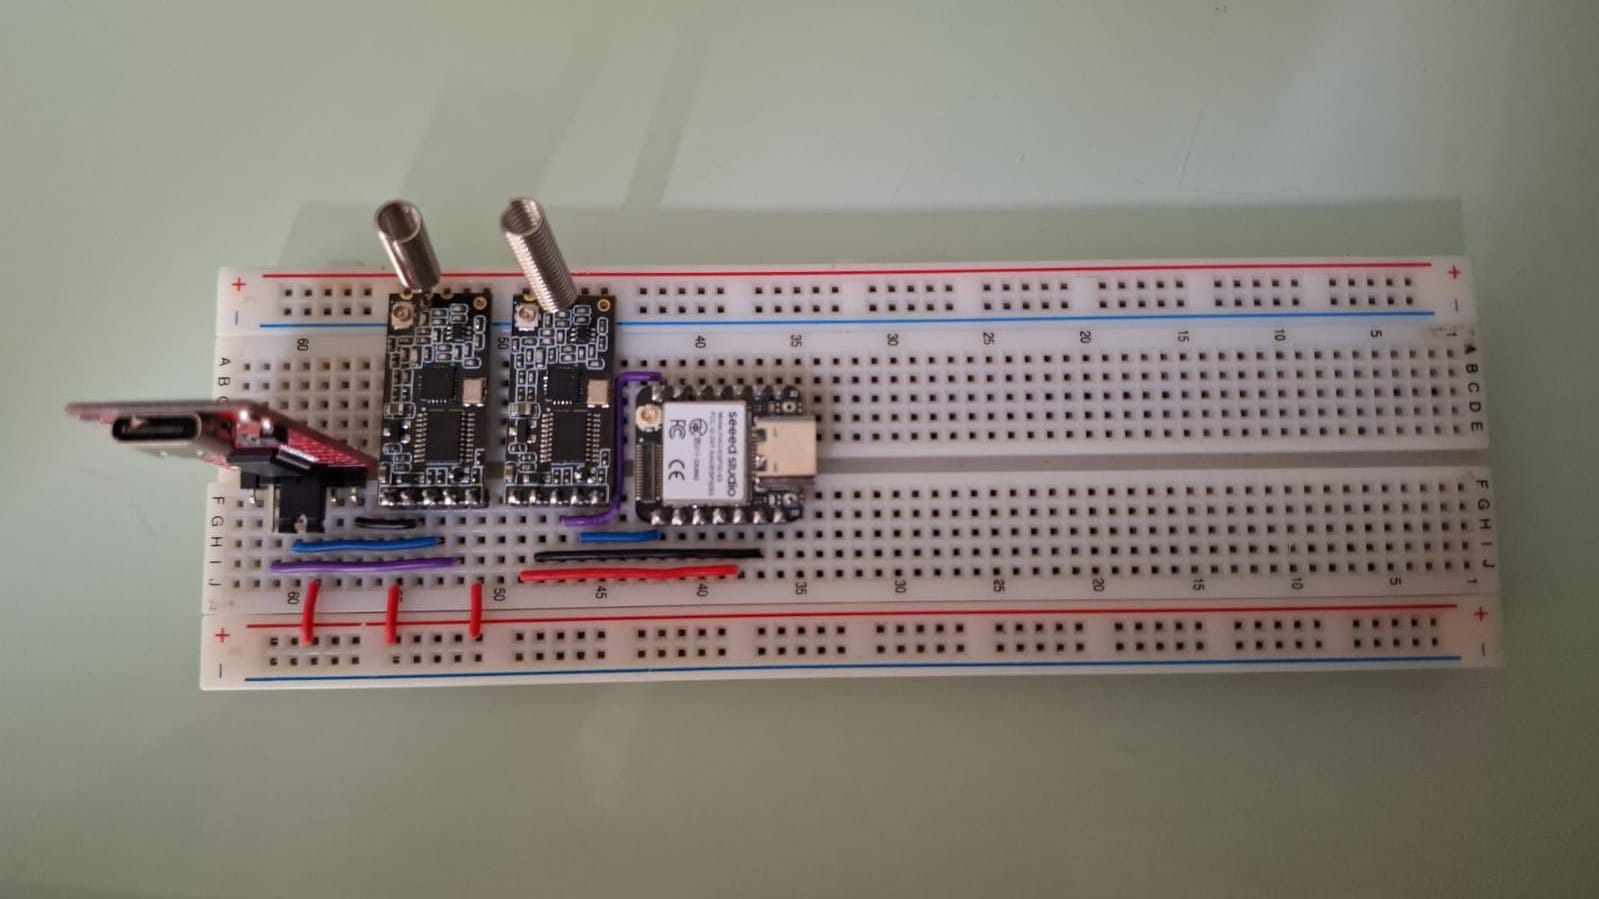
\includegraphics[width=0.9\textwidth]{e1.jpeg}
    \caption{Circuito final implementado en la protoboard.}
    \label{fig:e1_circuito}
\end{figure}


\subsection*{\fontsize{12}{17}\sffamily\selectfont Ejercicio 2}

Para el segundo ejercicio, se descargó el código fuente desde el proyecto ej\_uart el cual se encarga de establecer la comunicación serial. Es importante destacar que no fue necesario modificar ni una sola línea de código respecto al ejercicio de comunicación alámbrica, debido a que el enlace de radiofrecuencia con los módulos HC-12 opera de manera transparente.

La comunicación se lleva a cabo mediante la configuración del periférico UART de la ESP32-S3[cite: 7]. Primero, se inicializan los parámetros de comunicación a 9600 baudios, 8 bits de datos, sin paridad y un bit de parada[cite: 7]. Los pines asignados para esta tarea son el GPIO43 para transmisión (TX) y el GPIO44 para recepción (RX)[cite: 7].

\begin{lstlisting}[style=cstyle, caption={Configuración del puerto UART}, label={lst:configuracion}]
void uart_configurar(void)
{
    uart_config_t configuracion = {
        .baud_rate = UART_BAUD,
        .data_bits = UART_DATA_8_BITS,
        .parity    = UART_PARITY_DISABLE,
        .stop_bits = UART_STOP_BITS_1,
        .flow_ctrl = UART_HW_FLOWCTRL_DISABLE,
    };
    uart_param_config(UART_PUERTO, &configuracion);
    uart_set_pin(UART_PUERTO, PIN_TX, PIN_RX,
        UART_PIN_NO_CHANGE, UART_PIN_NO_CHANGE);
    uart_driver_install(UART_PUERTO, 256, 256, 0, NULL, 0);
}
\end{lstlisting}

En cuanto a la transmisión, el microcontrolador calcula periódicamente un valor correspondiente a una onda senoidal, escalado entre 0 y 255. Este byte se envía a través del puerto utilizando la función \texttt{uart\_write\_bytes}. A esta función se le pasa la dirección de memoria de la variable (\texttt{\&valor\_enviado}) dado que está diseñada de forma genérica para mandar bloques de datos mediante punteros.

\begin{lstlisting}[style=cstyle, caption={Transmisión de datos (Tx)}, label={lst:transmision}]
    // ejemplo 1: onda senoidal, un byte (0-255)
    uint8_t valor_enviado = (uint8_t)(127 + 127 * sin(angulo));
    uart_write_bytes(UART_PUERTO, &valor_enviado, 1);
    angulo += 0.2;
    if (angulo > DOS_PI) {
        angulo = 0;
    }
\end{lstlisting}

Simultáneamente, la ESP32-S3 se mantiene a la escucha de datos entrantes en el bus serial. Mediante la función \texttt{uart\_read\_bytes}, se lee el buffer de recepción y la función emplea el puntero \texttt{\&valor\_recibido} para escribir el dato entrante directamente en esa dirección de memoria. Si el programa detecta que el byte recibido equivale a 128 (\texttt{VALOR\_PRENDE}), el LED integrado de la tarjeta XIAO se enciende; con cualquier otro valor, se mantiene apagado. Este proceso se repite en un ciclo infinito con retardos de 500 milisegundos[cite: 7].

\begin{lstlisting}[style=cstyle, caption={Recepción de datos y control de actuador (Rx)}, label={lst:recepcion}]
    // recibir: prender o apagar el LED
    uint8_t valor_recibido;
    int bytes_leidos =
        uart_read_bytes(UART_PUERTO, &valor_recibido, 1, 0);
    if (bytes_leidos > 0) {
        if (valor_recibido == VALOR_PRENDE) {
            gpio_set_level(PIN_LED, LED_PRENDIDO);
        } else {
            gpio_set_level(PIN_LED, LED_APAGADO);
        }
    }
    vTaskDelay(pdMS_TO_TICKS(500)); // periodo: 500 ms
\end{lstlisting}

\subsection*{\fontsize{12}{17}\sffamily\selectfont Ejercicio 3}

Antes de validar el funcionamiento, es importante tener en cuenta que en sistemas operativos como linux, los archivos de dispositivos seriales (como \texttt{/dev/ttyACM0} o \texttt{/dev/ttyUSB0} utilizados por el convertidor TTL-USB o la tarjeta ESP32) son son propietarios de el usuario root y de un grupo llamado \texttt{dialout}. Por lo tanto, para no tener problemas de permisos al abrir el puerto serial, es necesario agregar a nuestro usuario al grupo \texttt{dialout} mediante el comando \texttt{sudo usermod -a -G dialout \$USER} y posteriormente cerrar sesión y volver a iniciar. Con este cambio, la aplicación SerialTest puede abrir el puerto serial sin que ocurra algun error en el acceso.

Para comprobar el funcionamiento del sistema, se instalo el software de SerialTest para monitorear la comunicación entre la computadora y el módulo HC-12 conectado a la ESP32-S3. Para ello, desde la aplicación SerialTest, se seleccionó el puerto /dev/ttyUSB0 correspondiente al convertidor USB a UART y se seleccionó la opción de open para configurar la comunicación a 9600 baudios, 8 bits de datos, sin paridad y un bit de parada.

\begin{figure}[H]
    \centering
    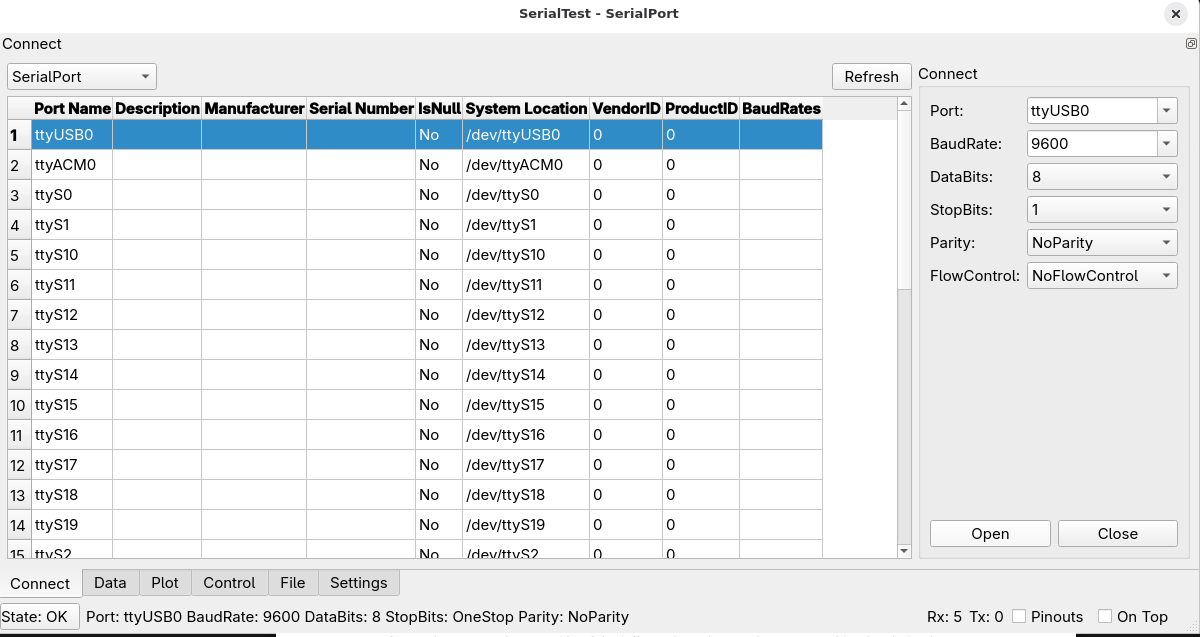
\includegraphics[width=0.9\textwidth]{e3_1.png}
    \caption{Configuración de la comunicación serial en la aplicación SerialTest.}
    \label{fig:e3_circuito}
\end{figure}

Una vez configurado el puerto serial, se abre la ventana de DATA para visualizar los datos que se estan recibiendo desde la ESP32-S3. En la siguiente imagen se puede observar que el valor recibido es una onda senoidal que oscila entre 0 y 255, tal como se esperaba. Además, al enviar un valor de 128 desde la ESP32-S3, el LED integrado de la tarjeta XIAO se enciende, confirmando que la comunicación bidireccional funciona correctamente.

\begin{figure}[H]
    \centering
    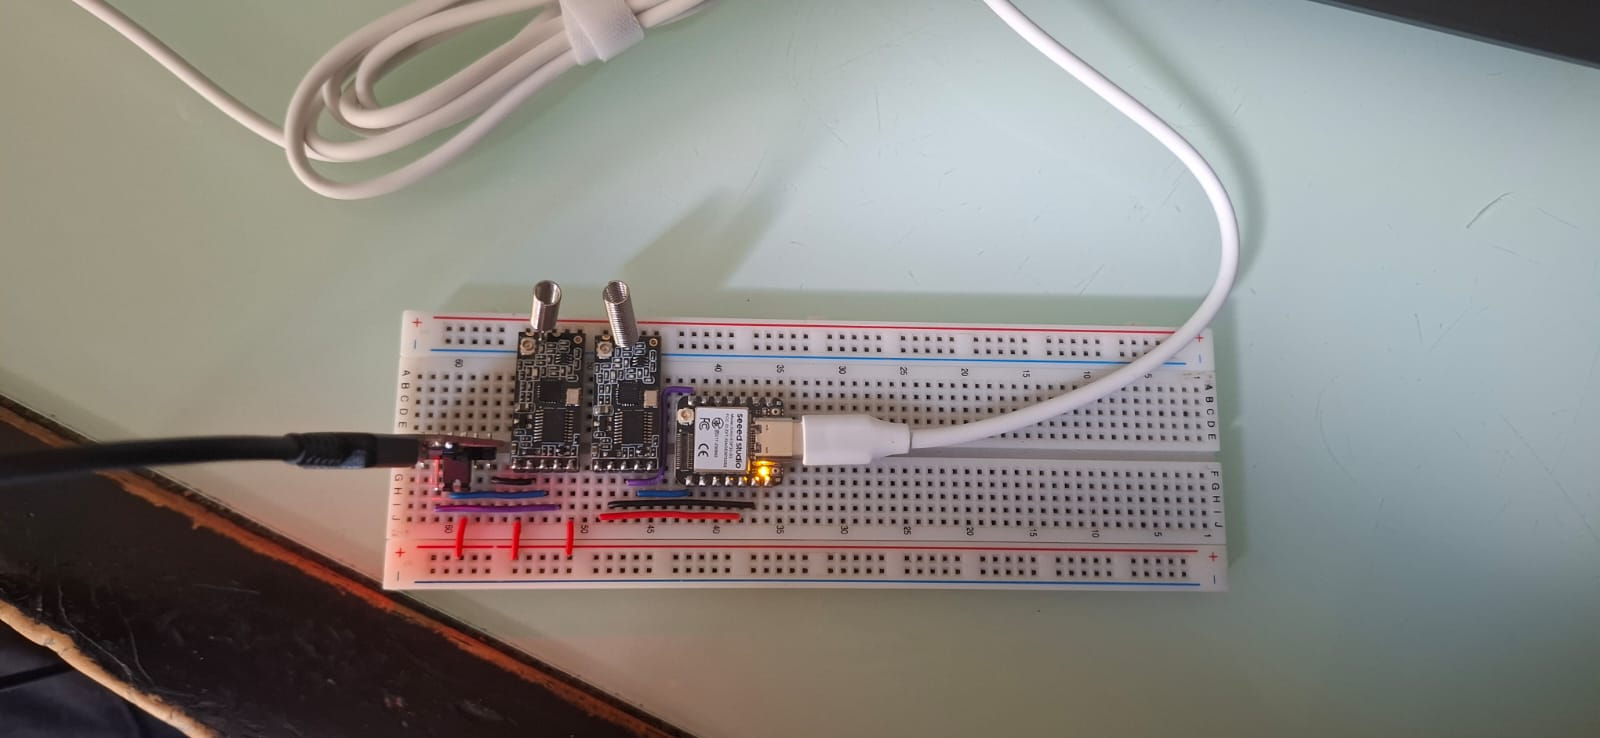
\includegraphics[width=0.8\textwidth]{e3_2.jpeg}
    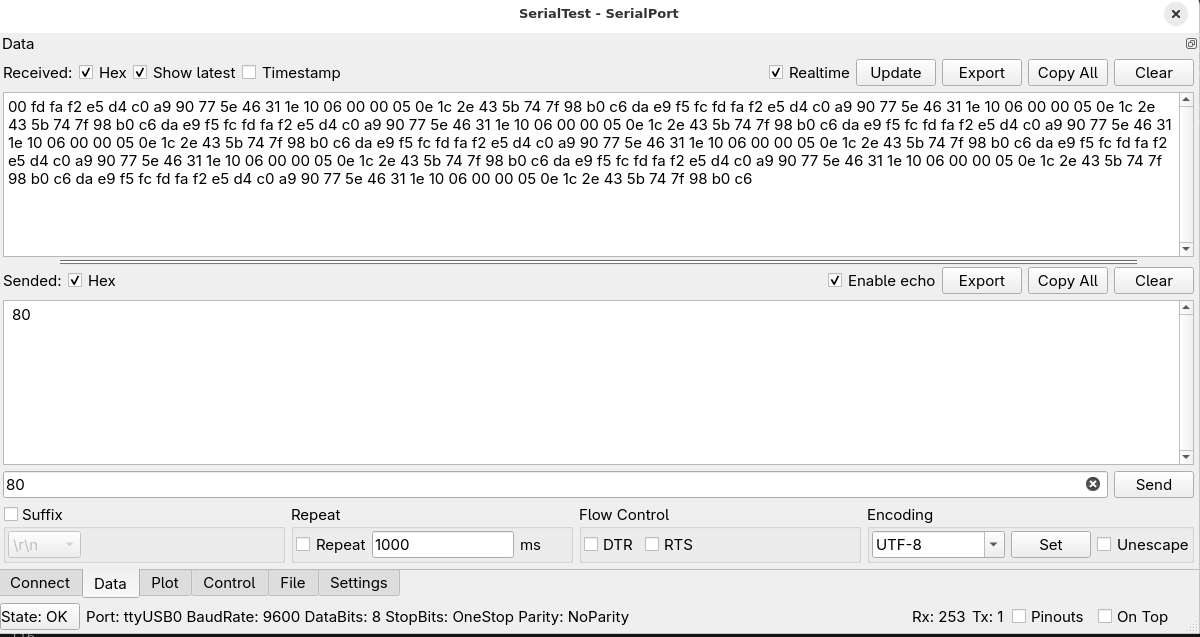
\includegraphics[width=0.8\textwidth]{e3_3.png}
    \caption{Verificación del encendido del LED integrado de la tarjeta XIAO ESP32-S3 al recibir el valor 128 desde la computadora.}
    \label{fig:e3_verificacion}
\end{figure}

Como puede observarse en la captura de pantalla de la aplicación SerialTest, la comunicación inalámbrica mediante los módulos HC-12 funciona correctamente, permitiendo la transmisión y recepción de datos entre la computadora y la tarjeta XIAO ESP32-S3. Ya que al enviar el valor de 128 (80 en hexadecimal) desde la ESP32-S3, el LED integrado de la tarjeta se enciende. Por ota parte, al enviar cualquier otro valor, el LED se mantiene apagado, confirmando que la comunicación bidireccional es estable y confiable.

\begin{figure}[H]
    \centering
    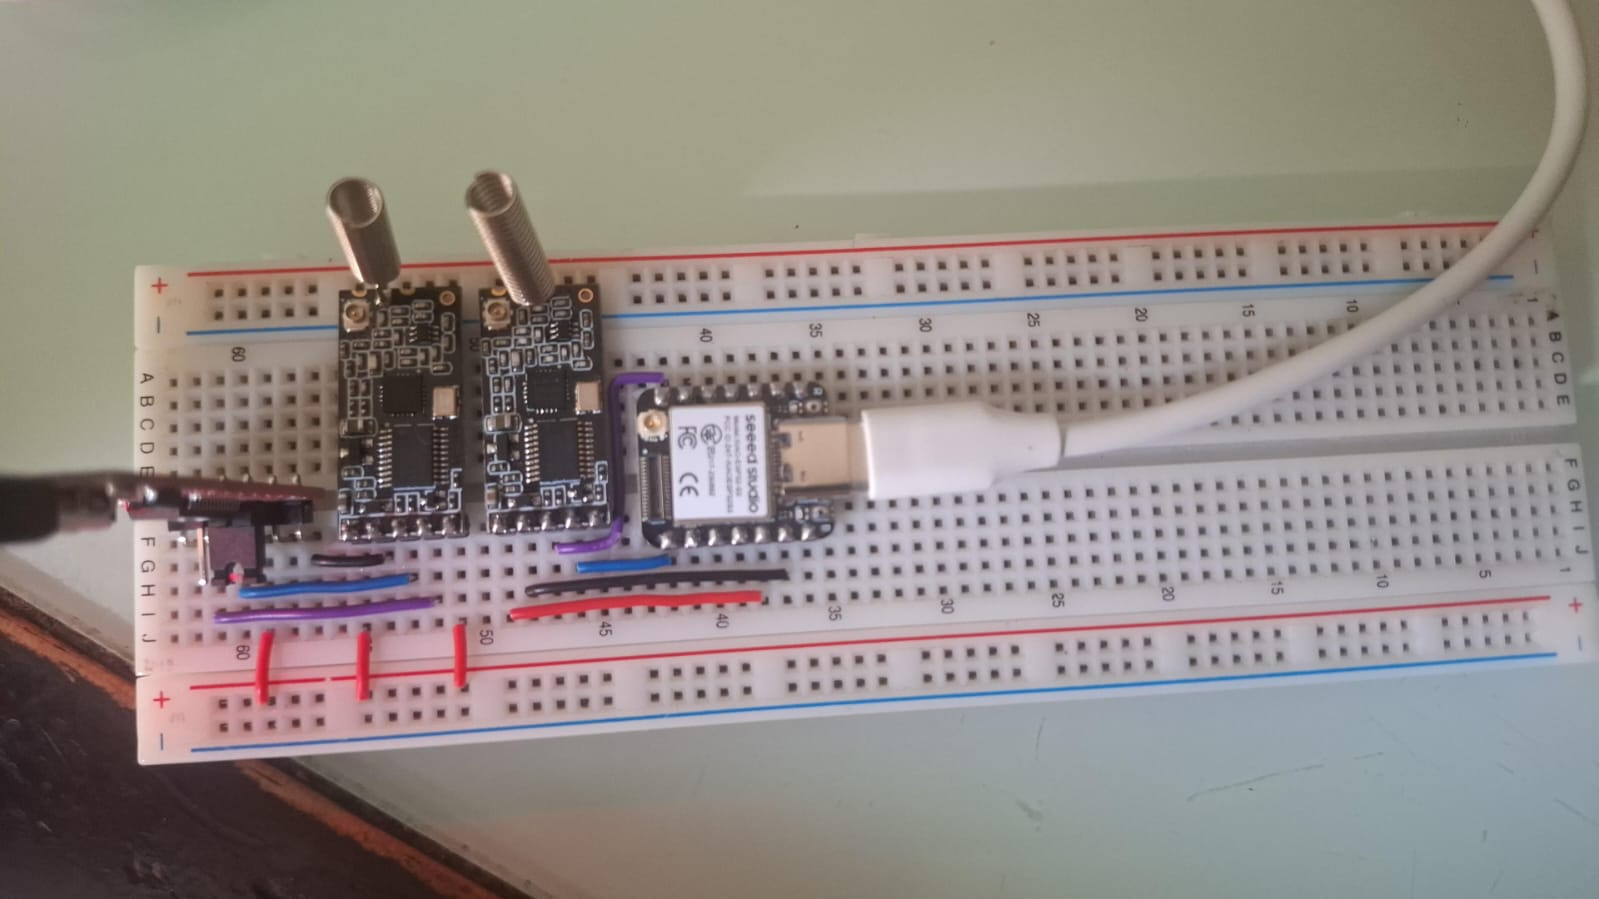
\includegraphics[width=0.8\textwidth]{e3_5.jpeg}
    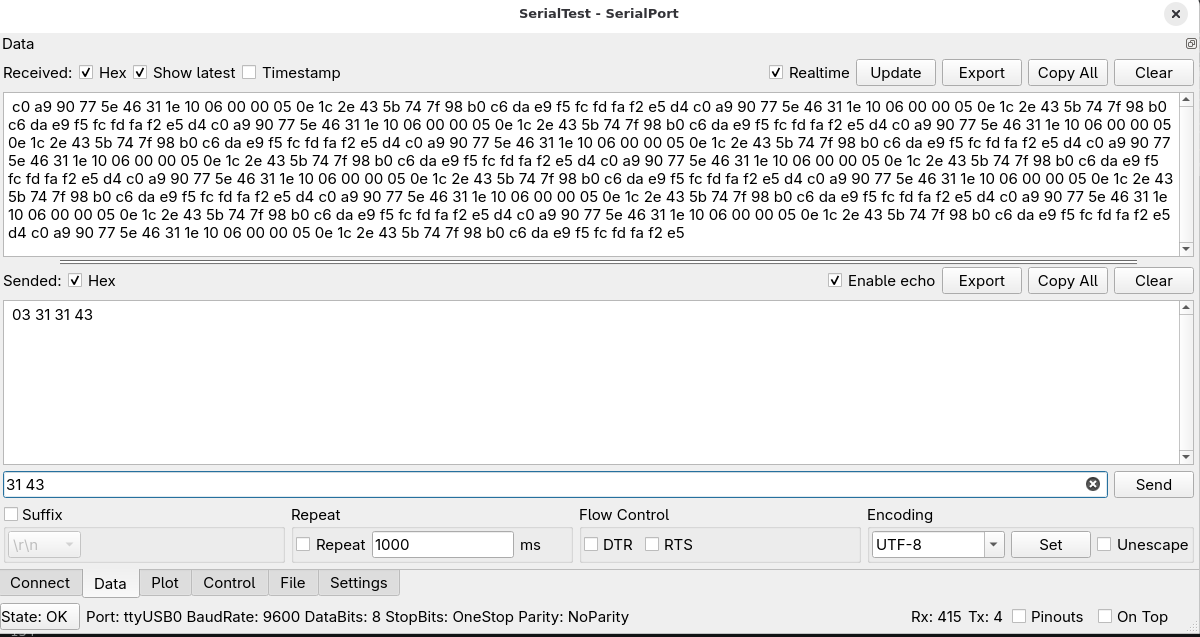
\includegraphics[width=0.8\textwidth]{e3_6.png}
    \caption{Verificación del apagado del LED integrado de la tarjeta XIAO ESP32-S3 al recibir un valor diferente a 128 desde la computadora.}
    \label{fig:e3_apagado}
\end{figure}

Para comprobar que la recepción de datos ocurre cada 500 milisegundos, se seleccionó la opción de "Timestamp" en la ventana de DATA de la aplicación SerialTest. Esto permite visualizar la hora exacta en que se reciben los datos, confirmando que la comunicación es periódica y estable.

\begin{figure}[H]
    \centering
    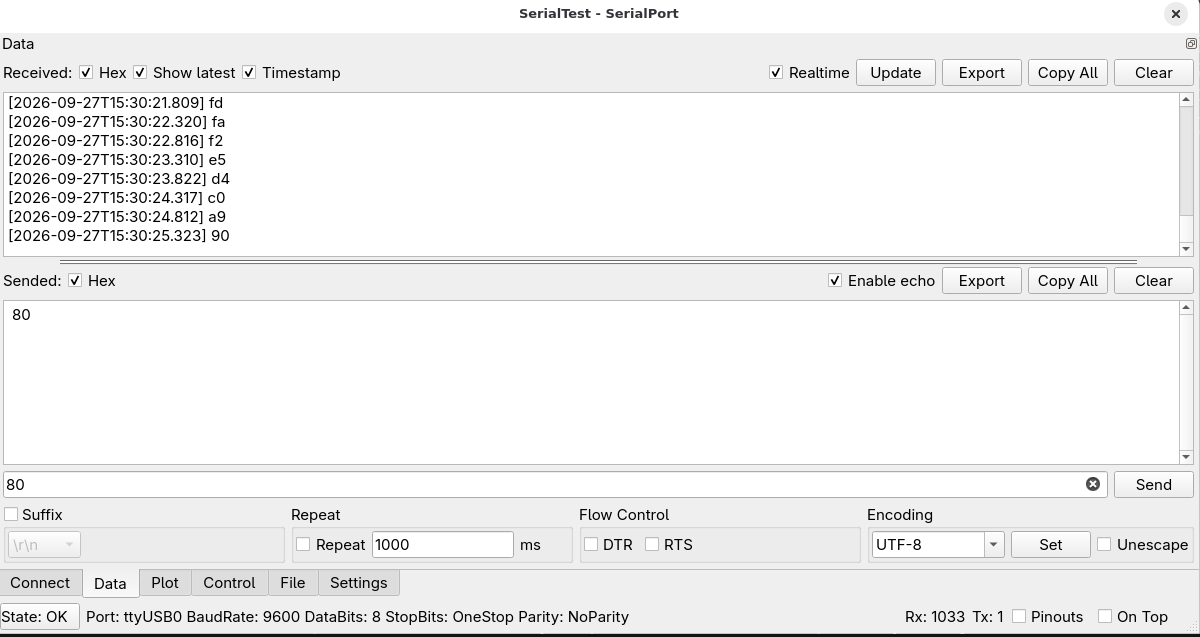
\includegraphics[width=0.8\textwidth]{e3_4.png}
    \caption{Verificación de la periodicidad de la recepción de datos cada 500 ms.}
    \label{fig:e3_periodicidad}
\end{figure}

Finalmente, para probar el alcance de la comunicación inalámbrica, se realizó una prueba de distancia entre los dos HC-12. Para ello, se colocaron en diferentes habitaciones de la casa.

\begin{figure}[H]
    \centering
    % Foto de la computadora (arriba)
    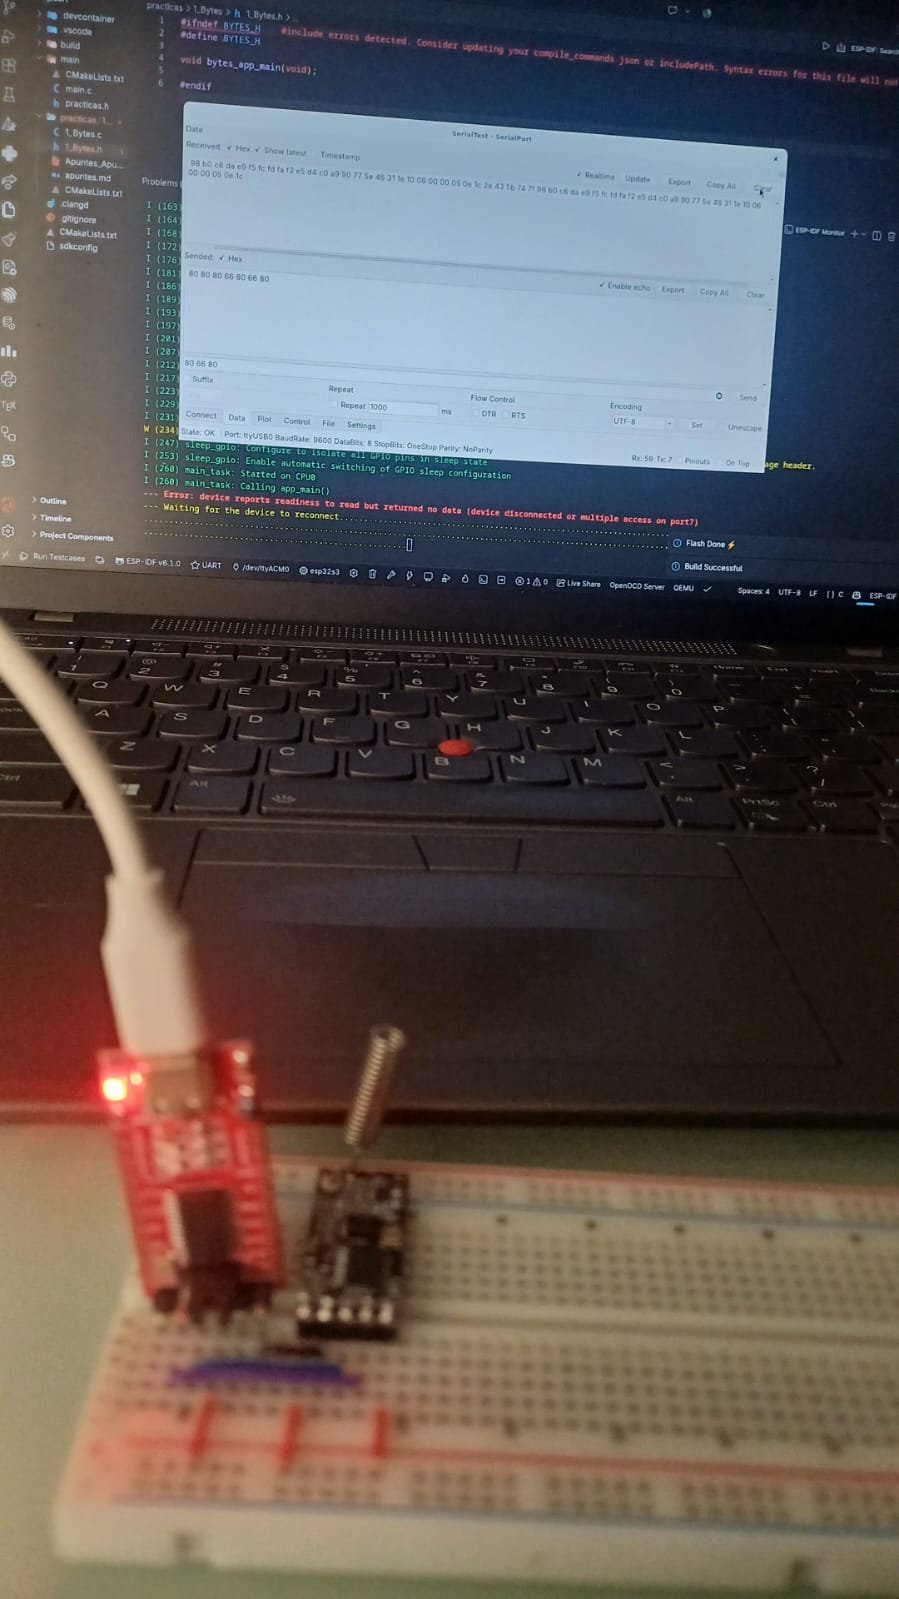
\includegraphics[width=0.3\textwidth]{e3_7.jpeg} \\[1em] % El \\ hace el salto de línea y [1em] agrega separación vertical
    
    % Fotos de los celulares (abajo)
    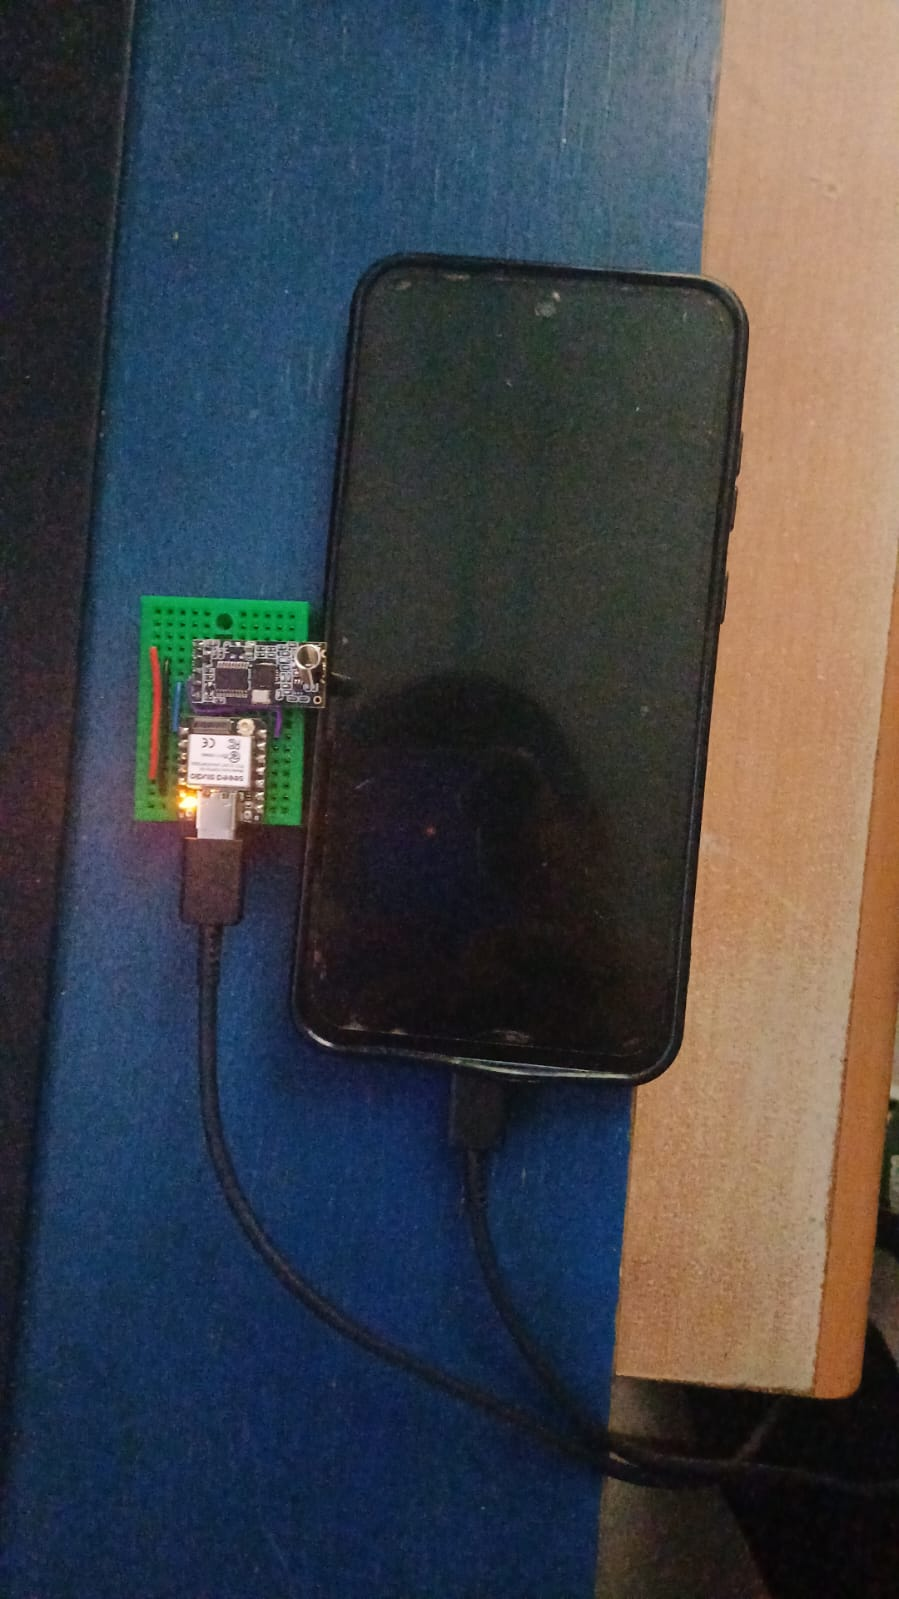
\includegraphics[width=0.25\textwidth]{e3_8.jpeg} \hspace{0.5cm} % \hspace agrega separación horizontal entre fotos
    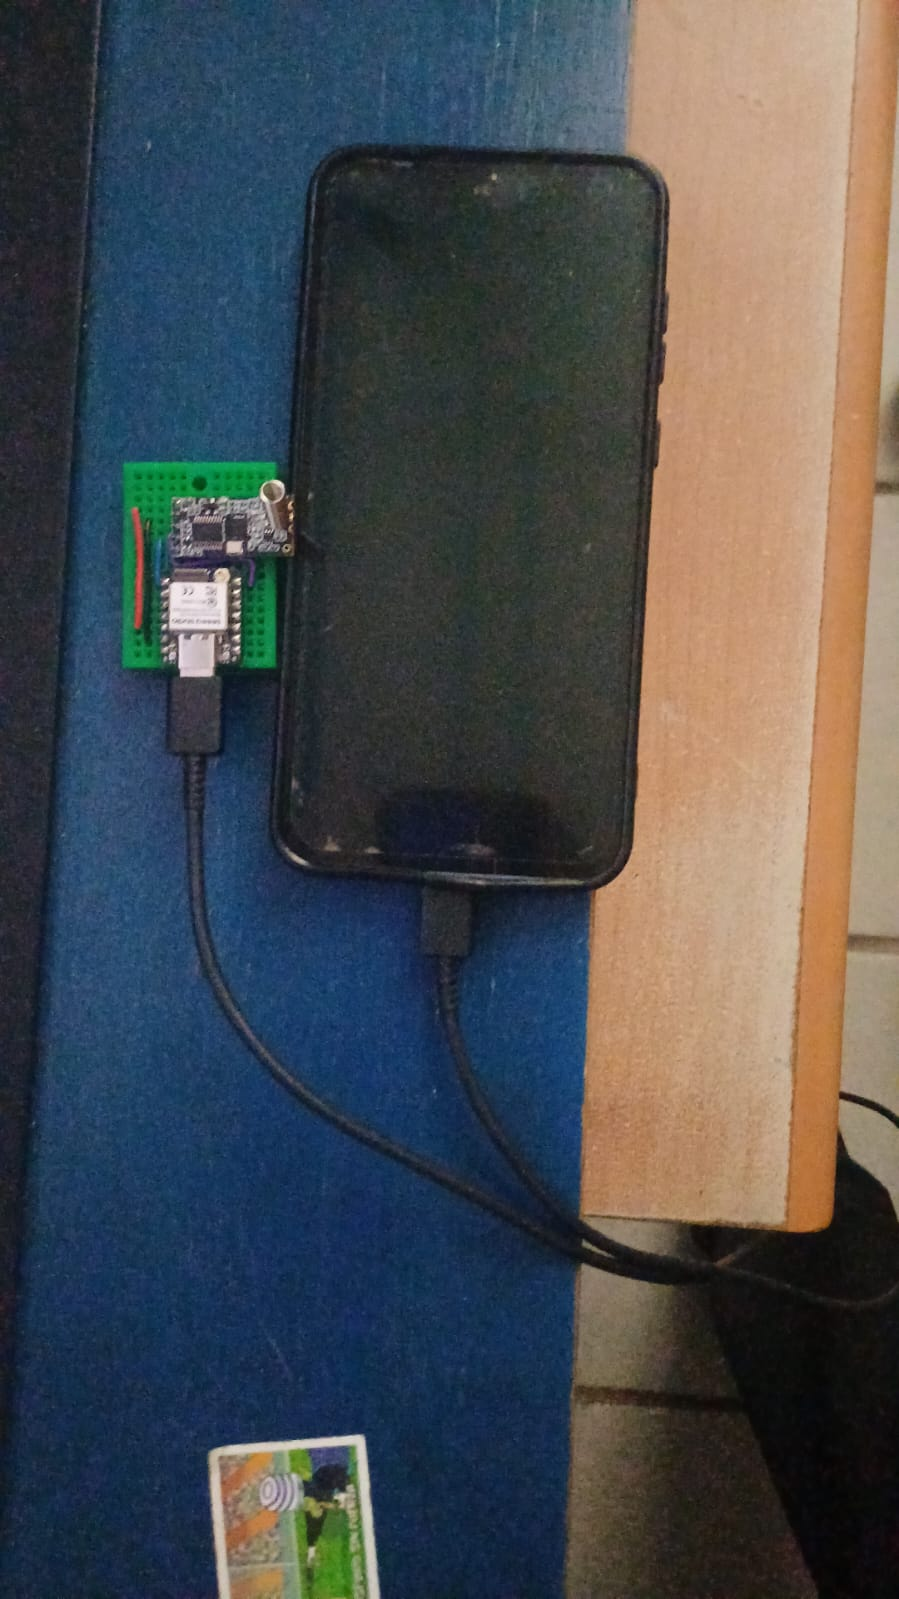
\includegraphics[width=0.25\textwidth]{e3_9.jpeg}
    
    \caption{Prueba de alcance de la comunicación inalámbrica entre los módulos HC-12 en diferentes habitaciones.}
    \label{fig:e3_alcance}
\end{figure}

Como puede verse a pesar de encontrarse alejadas un aproximado de 8 metros y con paredes de por medio, la comunicación entre los módulos HC-12 se mantiene estable y confiable, pues al enviar el valor de encendido (128) el cambio resultaba inmediato en el LED integrado de la tarjeta XIAO ESP32-S3, confirmando que la comunicación bidireccional funciona correctamente incluso a esa distancia y con obstáculos.

\section*{\centering \fontsize{14}{17}\sffamily\selectfont Análisis}

Como se documentó en el Ejercicio 2, el aspecto más destacable de esta implementación es que no se tuvo que modificar ni una sola línea del código fuente de la ESP32-S3 en comparación con la implementación alámbrica. Esto se justifica debido a que los módulos HC-12 operan en lo que se conoce como modo transparente. Para el microcontrolador, conectarse a los pines RX y TX del HC-12 es completamente indistinguible de estar conectado a un cable UART tradicional; toda la modulación, empaquetado y transmisión de radiofrecuencia es gestionada internamente por el hardware del módulo.

En las pruebas físicas, se comprobó que la comunicación seguía siendo confiable incluso a una distancia aproximada de 8 metros y con paredes de por medio. Esta fiabilidad frente a obstáculos es característica de los transceptores sub-GHz (banda de 433 MHz típica de los HC-12), cuyas ondas electromagnéticas tienen una gran capacidad de penetración en interiores, superando en este aspecto a tecnologías de mayor frecuencia como el Wi-Fi.

Para que este enlace funcione, es un requisito absoluto que ambos módulos se encuentren en el mismo canal de frecuencia y velocidad. Si los HC-12 quedaran configurados en canales distintos, la comunicación fallaría por completo, ya que un módulo estaría transmitiendo en una frecuencia que el otro no está escuchando. Afortunadamente, estos módulos vienen configurados de fábrica para operar en el mismo canal predeterminado. Si en un entorno con interferencias se necesitara cambiar el canal, bastaría con poner en estado bajo (GND) el pin SET, lo que saca al módulo del modo transparente y lo entra al modo de comandos AT. Una vez en este modo, se envía el comando \texttt{AT+Cxxx} (donde \texttt{xxx} es el número del canal, por ejemplo, \texttt{AT+C005}) para reconfigurarlo.

\section*{\centering \fontsize{14}{17}\sffamily\selectfont Conclusiones}

La transición de una comunicación alámbrica a una inalámbrica presenta ventajas evidentes, siendo la principal la eliminación de las barreras físicas. Esto permite una total movilidad del prototipo y facilita el aislamiento eléctrico entre la etapa de control (PC) y el sistema integrado (microcontrolador). Sin embargo, también conlleva desventajas frente al UART tradicional: el medio inalámbrico es susceptible a interferencias electromagnéticas externas, el alcance está limitado por el entorno físico, y se requiere circuitería y alimentación adicional en el extremo remoto para hacer funcionar el módulo de radio.

A nivel de seguridad, la comunicación implementada presenta una vulnerabilidad crítica: los datos viajan "en texto claro" a través de un medio público y compartido. Dado que el sistema solo verifica si el valor recibido es 128 para encender el actuador (LED)[cite: 12, 13], cualquier persona dentro del rango de cobertura que tenga un módulo en el mismo canal podría realizar un ataque de inyección de datos para encender o apagar el dispositivo sin autorización, o bien, interceptar pasivamente la información que transmite el microcontrolador.

Para reducir estos riesgos sin perder la utilidad del enlace de RF transparente, es imperativo implementar seguridad a nivel de software. Esto se lograría aplicando algoritmos de cifrado a los bytes antes de mandarlos por la función \texttt{uart\_write\_bytes}[cite: 12, 13] y descifrándolos al recibirlos, o bien, diseñando un protocolo de tramas que incluya una dirección lógica del destinatario y sumas de verificación (checksums) para descartar comandos de emisores no válidos.

% \section{Bibliografía}

\begin{biblio}
	% for: https://sistemasmultibasededatos.blogspot.com/
	\item Esquivel Martinez H. (2021, Noviembre 28). \textit{SISTEMAS MULTIBASE DE DATOS} [Online]. Disponible en: \newline \textcolor{blue}{\underline{\url{https://sistemasmultibasededatos.blogspot.com/}}}
\end{biblio}

\newpage
\textbf{NOTA: Si se desea consultar el código fuente completo del proyecto, se puede acceder al repositorio de GitHub en la siguiente dirección:} \url{https://github.com/lethalSopaper/laboratorio_sistemas_embebidos}

\end{document}
